\chapter{Background: Classic Flag Algebras}
\label{chap:classic_flags}

In section \ref{sec:flag_algebras} we will briefly introduce Razborov's
flag algebras as they apply to
graphs. If the reader is already familiar with flag algebras this section can be skipped.

In section \ref{sec:semidefinite_method} we will discuss how the semidefinite method is applied
to flag algebras.
The method we use is slightly different to the method used in other works
(e.g. \cite{silvaFlagAlgebrasFirst2016}) but is more easily adapted to our new framework. This
section may be of interest even to a reader familiar with flag algebras.

Finally in section \ref{sec:coloured_graphs} we will introduce \textit{coloured graphs} as combinatorial
objects with their own structure. These will help us unlock the full potential of
our local flags in section TODO.

\section{Flag Algebras}
\label{sec:flag_algebras}

All the following definitions, theorems etc.
are concepts from \cite{razborovFlagAlgebras2007}, rephrased
to focus only on the simple graph case.
For similar introductions to flag algebras we point the reader to
\textit{Flag Algebras: A First Glance} by Silva, Filho and Sato
\cite{silvaFlagAlgebrasFirst2016} and \textit{A Brief Introduction to Flag Algebra} by Qi
\cite{qiBriefIntroductionFlag}.

We saw in the \hyperref[sec:motivating_example]{motivating example} above that we want
to construct a symbolic algebra out of small graphs with some nice properties:
\begin{itemize}
    \item We would like the algebraic operations
        to be easily computable\footnote{at least with some computer software assistance}.
    \item We want the algebra to describe true relationships about densities in large graphs.
        i.e. If $A + B \geq C^2\cdot D$ is a true statement in our algebra
        then that must imply that $p(A; G) + p(B; G) \geq p(C; G)^2 \cdot p(D; G)$ for any $G$ large
        enough.
\end{itemize}

When we defined the induced count $c(F; G)$ we counted all possible instances of $F$
in $G$; Sometimes we want to only consider a subset of those instances, those where
we force some fixed vertices in $F$ to be mapped to some fixed vertices in $G$.
(e.g. if we count the copies of $\edge$ in $G$ where we force the first vertex to be mapped
to some fixed $v\in V(G)$ then $c(F; G) = \deg v$). This motivates the last desirable
properties of our algebra.

\begin{itemize}
    \item We would like our symbolic algebra to be able to capture densities where we have fixed
        some vertices.
    \item We want to be able to relate these "fixed" densities to the un-fixed densities.
\end{itemize}

Razborov's flags algebras give us all these nice properties. This section covers the
basic formalisms; Introducing a density function which accounts for pre-fixing some vertices,
defining what it means for something to hold "for large graphs", defining the actual
flag algebras with their properties, introducing an ordering $\geq$ and finally
covering the averaging operator which
relates "fixed vertex" densities to their un-fixed counterparts.

\subsection{Flags}

The fundamental object of our algebra is the \textit{flag} which is a partially
labelled graph, meaning some of the vertices of the graph have integer labels assigned to
them\footnote{The term flag apparently refers to the fact that some of the graph is fixed and the rest hangs loose, like a flag in the wind}. There may be no labelled vertices.
The labelled vertices will correspond then to those vertices which are fixed when we count
copies of the graph in some larger graph.

The \textit{type} of the flag is the subgraph induced by the labelled vertices.
In figure \ref{fig:flags-types} we see some example flags and their types. The labelled vertices
are represented visually with a partially filled vertex.

\begin{figure}[h]
    \centering
    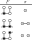
\includegraphics{flags-types-example}
    \caption{Example flags and their types}
    \label{fig:flags-types}
\end{figure}

We give the formal definitions:

\begin{definition}[Type]
    \label{def:type}
    A \textbf{type} $\sigma$ of size $k$ is a graph with vertex set $[k]$. We write
    $|\sigma|$ to denote the size of the underlying graph. We write
    $\emptyset$ to denote the type consisting of the empty graph.
\end{definition}
\begin{definition}[$\sigma$-Embedding]
    Given a type $\sigma$ and a graph $F$, a \textbf{$\sigma$-embedding} is an injective
    function $\theta\colon[|\sigma|]\to V(F)$ which is a graph isomorphism between
    $\sigma$ and $F[\im \theta]$.
\end{definition}
\begin{definition}[$\sigma$-Flag]
    \label{def:sigma_flag}
    A \textbf{$\sigma$-flag} is a tuple $(F, \theta)$ where $\theta$ is an $\sigma$-embedding
    into $F$.
    If the embedding is implicit (e.g. if $\sigma=\emptyset$) we often drop the
    $\theta$ from the notation.
\end{definition}

\begin{note}
    A type $\sigma$ is implicitly itself a $\sigma$-flag when taken with the
    identity embedding $\id\colon [|\sigma|] \to [|\sigma|]$. We often use this fact
    implicitly.
\end{note}

We then say that two flags are isomorphic if there is a graph isomorphism between the underlying
graphs which preserves the labels.
\begin{definition}[Flag Isomorphism]
    $f\colon V(F) \to V(F')$ is a $\sigma$-flag isomorphism
    from $(F,\theta) \to (F', \theta')$ if it is graph isomorphism $F \to F'$ such that
    $f(\theta(i)) = \theta'(i)\ \forall\ i\in [|\sigma|].$ We can
    write $(F,\theta)\cong (F',\theta')$ if such an $f$ exists.
\end{definition}

Now that we have a definition for flags we can build on our induced density function from
the introduction.

\subsection{Induced Counts and Density}

In the introduction we defined the induced count $c(F; G)$ to be the number of
$U\subseteq V(F)$ such that $G[U] \cong F$. If both $F$ and $G$ are partially labelled
and have the same type (so are "compatible"), then we
can ask how many copies of $F$ are there in $G$ where the fixed part of $F$ maps to the
fixed part in $G$.

\begin{definition}[Induced Count]
    \label{def:induced_count}
    Fix two $\sigma$-flags $(F,\theta), (G,\eta).$ We define the induced count of $(F,\theta)$ in
    $(G,\eta)$ written $c((F,\theta); (G,\eta))$
    as the number of subsets $\im(\eta)\subseteq U\subseteq V(G)$ such that
    $(F,\theta) \cong (G[U], \eta)$.\footnote{Where we restrict the codomain of $\eta$ appropriately}
\end{definition}

We can extend this notion of counting how many copies of $F$ there are in $G$ to multiple flags,
asking how many tuples of disjoint copies of $F_1, \dots, F_t$ are there in $G$ (where
disjoint means vertex-disjoint apart from the fixed labelled vertices).

Precisely we define $c(F_1, \dots, F_t; G)$ to be the number of
$U_1, \dots, U_t\subseteq V(G)$ such that $\im\eta = U_i \cap U_j\ \forall\ i, j \in [t]$ where
$i\neq j$ and $(F_i, \theta_i) \cong (G[U_i], \eta)$ for all $i\in [t].$

Note that if $c(F_1, \dots, F_t; G) > 0$ we know that $G$ must be large enough to fit
disjoint copies of $F_1, \dots, F_t$ leading us to the following definition.

\begin{definition}[Fit]
    We say $\sigma$-flags $F_1, \dots, F_t$ \textbf{fit} in $\sigma$-flag $G$ if
    $|G|-|\sigma| \geq \sum_{i=1}^t |F_i|-|\sigma|$.
\end{definition}

\begin{example}
    Consider the type $\sigma=\vertex$, a single vertex. Any $\sigma$-flag $(G,\eta)$ is
    just a graph with a specific distinguished vertex (the unique labelled vertex).

    Consider then the $\sigma$-flag $F=\edgemarked$, an edge with a single labelled vertex.
    For any $G$ with distinguished vertex $v$ we have $c(\edgemarked; G^v) = \deg_G(v)$.
    \footnote{$G^v$ is the $\vertex$-flag $(G,\theta)$ where $\theta(1)=v$.}

    Similarly, $c(\edgemarked, \edgemarked; G^v) = \binom{\deg(v)}{2}.$ This is as
    we are counting how many distinct pairs of vertices $(a, b)$ are there in $G$ such that
    $G[\{a, v\}] \cong \edgemarked$ and $G[\{b, v\}] \cong \edgemarked$.
    In other words, how many distinct pairs of vertices are there connected to
    $v$, which is clearly $\binom{\deg(v)}{2}.$
\end{example}

Now we can define the induced density by normalising the induced count by the max
possible number of such non-overlapping $t$-tuples.

\begin{definition}[Induced Density]
    \label{def:induced_density}
    Given $\sigma$-flags $F_1, \dots, F_t$ and $G$ define the \textbf{induced density} of
    $F_1, \dots, F_t$ in $G$ as:
    \[
    p(F_1, \dots, F_t; G)
    := \frac{c(F_1, \dots, F_t; G)}{
    \binom{|G|-|\sigma|}{|F_1|-|\sigma|, \dots,|F_t|-|\sigma|, R}}
    \]
    where we use multinomial coefficient notation with
    $R=(|G|-|\sigma|)-\sum_{i=1}^t |F_i|-|\sigma|$.
\end{definition}

\begin{note}
    Again, as in the \hyperref[sec:motivating_example]{motivating example in the introduction},
    we can interpret $p(F_1, \dots, F_t; G)$ in a precise probabilistic way.
    $p(F_1, \dots, F_t; G)$ is exactly the probability that
    $(F_i, \theta_i) \cong (G[U_i], \eta)\ \forall\ i\in[t]$ where
    $U_1, \dots, U_t \subseteq V(G)$ is a uniformly random $t$-tuple of subsets such that
    $U_i \cap U_j = \im \eta\ \forall i, j \in [t], i \neq j$.
\end{note}

\subsection{Graph Classes}

Often, we want to limit our view to a subset of all possible graphs. For example, we
will want to consider only triangle-free graphs when proving Mantel's theorem (TODO REF).

We pick some class of graphs $\Gcl$. For Razborov's flag algebras we assume that
$\mathcal{G}$ is hereditary, meaning it is closed under taking induced subgraphs. This will change
when we introduce our new local framework.

Then for any type $\sigma$ we write $\Gcl^\sigma$ for the set of all $\sigma$-flags up to
isomorphism. We write $\Gcl^\sigma_n$ for the set of all $\sigma$-flags of size $n$.
We generally assume $\Gcl^\sigma$ is infinite for any type $\sigma\in\mathcal{G}$.
If $\sigma=\emptyset$ we often skip the superscript and just refer to
$\Gcl$ or $\Gcl_n$.

From this point all definitions and results are relative to some fixed graph class
$\mathcal{G}$.

Given some graph class $\mathcal{G}^\sigma$ then we get the very power \textit{chain rule}.
\begin{lemma}[The Chain Rule, Lemma 2.2 \cite{razborovFlagAlgebras2007}]
    \label{lemma:chain_rule}
    If $F_1, \dots, F_t \in \Gcl^\sigma$ are $\sigma$-flags which fit in $G\in\Gcl^\sigma$
    then for all $1 \leq s \leq t$ and every $n$ such that
    $F_1, \dots, F_s$ fit into a $\sigma$ flag of size $n$ and a
    $\sigma$-flag and $F_{s+1}, \dots, F_t$ fit in $G$ we have:
    \[
    p(F_1, \dots, F_t; G) = \sum_{F \in \mathcal{G}^\sigma_n}
    p(F_1, \dots, F_s; F)p(F, F_{s+1}, \dots, F_t; G).
    \]
\end{lemma}

This chain rule is one of the crucial properties that we will lose when we define our
local flags framework.

\subsection{Limit Functionals}
\label{sec:limit_functionals}

We want to define our algebra such that the results it derives are true for large enough
flags. How do we make that precise?

Consider a sequence of $\sigma$-flags $(G_k)_{k\in\N}$ which is \textit{increasing}, meaning
the sequence $(|G_k|)_{k\in\N}$ is strictly increasing. Then for $F\in\Gcl^\sigma$
consider the function $\lim_{k\to\infty} p(F; G_k)$. We call a sequence of $\sigma$-flags
$(G_k)_{k\in\N}$ \textbf{convergent} if this limit exists for all $F\in\Gcl^\sigma$.
It is a result of Tychonoff's theorem that any increasing sequence of graphs contains a convergent
subsequence (as $[0,1]^{\Gcl^\sigma}$ is compact). For this reason it suffices to only
consider convergent sequences.

Now we can introduce the limit functional which precisely links our symbolic algebra
to it's underlying interpretation in terms of density functions.

\begin{definition}[Limit Functional]
    Given some convergent $\sigma$-flag sequence we construct the corresponding
    \textbf{limit functional} $\phi\colon \Gcl^\sigma \to [0,1]$
    as
    \[
        \phi(F) := \lim_{k \to \infty} p(F; G_k)
    \]
\end{definition}

We write $\Phi^\sigma$ for the collection of all limit functionals for type $\sigma$.

\begin{example}
    If we prove that $\phi(\edge) \leq \frac{1}{2}$ for all $\phi\in\Phi^\emptyset$
    where $\Gcl$ is the class of triangle free graphs, then we will have proved Mantel's theorem
\end{example}

We will see later that limit functionals give us exactly the interpretation of statements
in our algebra as asymptotic statements about densities.

\subsection{The Algebra}

We've described flags in detail, understanding a partially labelled flag and
the density functions they in some way represent. We would like to then formally
describe a symbolic structure on these flags such that relations in the structure describe true
relations about their associated density functions. As a start we want to be able
to describe linear combinations of flags, e.g. $\edge + \nonedge$ should in some
way represent $p(\edge; G) + p(\nonedge; G)$.

Take then the formal real vector space $\R\Gcl^\sigma$ for some fixed type $\sigma$,
this gives us a proper notion of these linear combinations of flags. We can then
linearly extend our density function $p$ to this space in the first argument giving
us a function $p\colon \R\Gcl^\sigma \times \Gcl^\sigma \to \R$ capturing that
$p(\edge + \nonedge; G) = p(\edge; G) + p(\nonedge; G) = 1$ and similar relations.

The chain rule (Lemma \ref{lemma:chain_rule}) tells us then that for any $F, G\in\Gcl^\sigma$
and $n \geq |F|$ we have $p(F; G) = \sum_{H \in \Gcl^\sigma_n}p(F; H)p(H; G)$. In
In particular $p(F; H)$ is just some real, computable number for each $H$ meaning
$p(F; G) - \sum_{H \in \Gcl^\sigma_n}p(F; H)p(H; G) = 0$ is a linear relation on
density functions which holds for all $F, G$. This tells us that in our algebra
any vector of the form $v = F - \sum_{H \in \Gcl^\sigma_n}p(F; H)H$ has the property
that $p(v; G) = 0$ for all $G\in\Gcl^\sigma$.

We can define the space $\mathcal{K}^\sigma$ as the span of vectors of the form
$F - \sum_{H \in \Gcl^\sigma_n}p(F; H)H$ for $F\in\Gcl^\sigma$, $n\geq |F|$ and
quotient out this relation from $\R\Gcl^\sigma$. Because $p(v; G) = 0$ for all
$v \in\mathcal{K}^\sigma, G \in\mathcal{G}$ our linear extension of $p$ is still well defined
on this space.

Not only is $p$ well defined on this space, we can now also
linearly extend any limit functional $\phi$ to be a function
$\phi\colon\R\Gcl^\sigma / \mathcal{K}^\sigma\to \R$.

\begin{example}
    If $\Gcl$ is the class of triangle free graphs then we know from our
    \hyperref[sec:motivating_example]{motivating example} that
    $p(\edge; G) = \frac{2}{3}p(\triangletwoedge; G) + \frac{1}{3}p(\triangleoneedge; G)$
    for all $G\in\mathcal{G}$. We would like this to translate to a relation like
    $\edge = \frac{2}{3}\triangletwoedge + \frac{1}{3}\triangleoneedge$.

    In the space $\R\Gcl^\emptyset / \mathcal{K}^\emptyset$ both the vectors $\edge$ and
    $\frac{2}{3}\triangleoneedge + \frac{1}{3}\triangleoneedge$ belong to the same
    coset, so they are indeed equal. Hence this space does capture this relationship.
\end{example}

However, linear combinations are not powerful enough. We also want to be able to make
statements about products of densities. Ideally we would be able to define a
product on vectors $f, g \in \R\Gcl^\sigma / \mathcal{K}^\sigma$ such that for any $G\in\Gcl^\sigma$
we have $p(f \cdot g; G) = p(f; G)\cdot p(g; G)$. Unfortunately we don't achieve the
ideal relation, but we do get the result asymptotically:
$\phi(f\cdot g) = \phi(f) \cdot \phi(g)\ \forall\ \phi\in\Phi^\sigma$.

\begin{definition}[$\sigma$ Flag Algebra]
    For fixed type $\sigma$ define the following product $\Gcl^\sigma \times \Gcl^\sigma \to \R\Gcl^\sigma / \mathcal{K}^\sigma$
    on $\sigma$-flags $F, G\in\Gcl^\sigma$.
    \[
        F \cdot G := \sum_{H \in \Gcl^\sigma_\ell} p(F, G; H) \cdot H
    \]
    for any $\ell \geq |F|+|G|-|\sigma|$.
    Extend this product then bilinearly to the space
    $\R\Gcl^\sigma \times \R\Gcl^\sigma$. This then induces a bilinear map
    $\R\Gcl^\sigma / \mathcal{K}^\sigma \times \R\Gcl^\sigma / \mathcal{K}^\sigma \to \R\Gcl^\sigma / \mathcal{K}^\sigma$.

    This is all well defined due to Lemma 2.4 in \cite{razborovFlagAlgebras2007}.
    This turns the space
    $\R\Gcl^\sigma / \mathcal{K}^\sigma$ into an algebra. We call this the
    \textbf{$\sigma$ flag algebra} $\Acl^\sigma$.

\end{definition}

This algebra is then associative, commutative and unital
(also lemma 2.4 in \cite{razborovFlagAlgebras2007}). Again this product can be computed
with a small number of $p(F, G; H)$ calculations where $F, G, H$ are fixed meaning this
is computable.

\begin{example}
    Let $\sigma=\vertex$. Then $(\edgemarked)\cdot(\nonedgemarked)$ is computed by
    choosing $\ell$ large enough so that $\edgemarked$ and $\nonedgemarked$ fit. We can
    pick $\ell = 3$. Then
    $\Gcl^\sigma_3=\{\trianglemarked, \triangletwoedgemarkedcentre, \triangletwoedgemarkedleft, \triangleoneedgemarkedtop, \triangleoneedgemarkedleft, \triangleemptymarked\}$
    and we can compute $p(\edgemarked, \nonedgemarked, G)$ for each $G\in\Gcl^\sigma_3$
    and find
    \[
        \begin{split}
            (\edgemarked)\cdot(\nonedgemarked)
            &= 0\cdot \trianglemarked + 0\cdot \triangletwoedgemarkedcentre
            + \frac{1}{2}\cdot \triangletwoedgemarkedleft + 0\cdot \triangleoneedgemarkedtop
            + \frac{1}{2} \cdot \triangleoneedgemarkedleft + 0\cdot \triangleemptymarked\\
            &= \frac{1}{2}\cdot \triangletwoedgemarkedleft
            + \frac{1}{2} \cdot \triangleoneedgemarkedleft.
        \end{split}
    \]
    (This isn't technically precise as we should be taking the coset).
    The product is bilinear so we can similarly compute expressions like:
    \[
        \begin{split}
            ((\edgemarked) - (\nonedgemarked))^2
            &= (\edgemarked)^2 - 2(\edgemarked)(\nonedgemarked) + (\nonedgemarked)^2\\
            &= (\trianglemarked + \triangletwoedgemarkedcentre)
            - 2(\frac{1}{2}\cdot \triangletwoedgemarkedleft
                + \frac{1}{2} \cdot \triangleoneedgemarkedleft)
            + (\triangleoneedgemarkedtop + \triangleemptymarked)\\
            &= \trianglemarked + \triangletwoedgemarkedcentre
            - \triangletwoedgemarkedleft - \triangleoneedgemarkedleft
            + \triangleoneedgemarkedtop + \triangleemptymarked
        \end{split}
    \]
\end{example}

Now we see the theorem which tells us why this product is useful:
\begin{theorem}[Theorem 2 \cite{silvaFlagAlgebrasFirst2016}]
    \label{thm:classic_product_lim}
    For fixed type $\sigma$, vectors $f, g\in \Acl^\sigma$ we have
    \[
        p(f; G)\cdot p(g; G) = p(f\cdot g; G) + O\left(\frac{1}{|G|}\right)
    \]
    where $G\in\Gcl^\sigma$.
\end{theorem}

What this theorem tells us is that our symbolic product corresponds to a valid product of
the underlying density functions in the limit, which we can use to prove asymptotic results.
We make this precise in the next section.

\begin{example}
    Returning to our example with $\sigma=\vertex$ and $F=\edgemarked$ we can compute that (choosing representative of cosets etc) we have
    $\edgemarked^2 = \trianglemarked + \triangletwoedgemarkedcentre.$ Let $G$ be a $\vertex$-flag
    with labelled vertex $v$. Then we know $c(\edgemarked; G^v) = \deg v$ from before.
    Then we can see that $c(\trianglemarked; G^v) + c(\triangletwoedgemarkedcentre; G^v)$ counts
    all possible ways of choosing pairs from the neighbourhood of $v$ hence
    $c\left(\trianglemarked; G^v\right) + c\left(\triangletwoedgemarkedcentre; G^v\right) = \binom{\deg v}{2}$.
    Therefore:
    \[
    \begin{split}
        p(\edgemarked; G^v)^2 - p(\edgemarked^2; G^v)
        &= \left(\frac{c(\edgemarked; G^v)}{|G|-1}\right)^2
            - p(\trianglemarked; G^v) - p(\triangletwoedgemarkedcentre; G^v)\\
        &= \left(\frac{\deg v}{|G|-1}\right)^2
            - \frac{c(\trianglemarked; G^v) + c(\triangletwoedgemarkedcentre; G^v)}{\binom{|G|-1}{2}}\\
        &= \left(\frac{\deg v}{|G|-1}\right)^2
            - \frac{\binom{\deg(v)}{2}}{\binom{|G|-1}{2}}\\
        &= \frac{\deg v}{(|G|-1)^2(|G|-2)}
            + \frac{\deg v}{(|G|-1)(|G|-2)}\\
        &= O\left(\frac{1}{|G|}\right).
    \end{split}
    \]
    as $\deg(v)\in O(|G|)$.
\end{example}

Now theorem \ref{thm:classic_product_lim} proves that our algebra does exactly capture
the algebraic behaviour of densities in the limit.
\begin{lemma}
    Any limit functional $\phi\colon\Acl^\sigma \to\R$ is an algebra homomorphism.
    Meaning for any $f, g\in\Acl^\sigma$ we have $\phi(f + g) = \phi(f) + \phi(g)$
    and $\phi(f\cdot g) = \phi(f) \cdot \phi(g)$.
\end{lemma}

\subsection{Positivity}

We want to introduce an order on our algebra so that statements like
$\edge \leq \triangleflag + \triangletwoedge + \triangleoneedge + \triangleempty$ have
meaning.

\begin{definition}[Positive]
    We say that $f\in\Acl^\sigma$ is \textbf{positive} if
    $\phi(f) \geq 0\ \forall\ \phi \in \Phi^\sigma$.

    We write this as $f \geq_{\Acl^\sigma} 0$ or most often just
    $f \geq 0$.
\end{definition}

\begin{example}
    All flags are positive elements of the algebra as densities are non-negative.
    Additionally any squared vector $f^2$ is positive as $\phi(f^2)=\phi(f)^2 \geq 0$.
    The zero vector is also positive.
\end{example}

We then extend this notation writing $f \geq g$ iff $f-g \geq 0$ meaning
$f \geq g$ iff $\phi(f) \geq \phi(g)$ for all $\phi\in\Phi^\sigma$.

\begin{note}
    Sometimes we will write something like $\edge \leq \frac{1}{2}$ which is technically
    not a valid statement. You can make this precise by thinking of $\frac{1}{2}$ as
    $\frac{1}{2}\emptyset$ as the empty graph always has $\phi(\emptyset) = 1$.
    This gives $\edge \leq \frac{1}{2}$ the intended meaning that
    $\phi(\edge) \leq \frac{1}{2}\ \forall\ \phi\in\Phi^\sigma$.
\end{note}

\begin{lemma}
    The set of positive elements of $\Acl^\sigma$ forms a convex cone, meaning it is
    closed under non-negative linear combination.

    We call this the semantic cone $\SemCone^\sigma$.
\end{lemma}

Now that we have positivity, and we know that the set of positive elements form a cone we can actually prove some results. In particular we know make formal the simple argument that
$p(\edge; G) \leq \frac{2}{3}$ for $G$ triangle free 
from our \hyperref[sec:motivating_example]{motivating example}.
\begin{example}
    Let $\Gcl$ be the class of triangle free graphs.

    We know that $F \geq 0$ for all flags $F$ ($\Gcl^\emptyset \subseteq \SemCone^\sigma$).
    We know that $\edge = \frac{2}{3}\triangletwoedge + \frac{1}{3}\triangleoneedge$
    and $\emptyset = \triangletwoedge + \triangleoneedge + \triangleempty$
    as they are in the same cosets (equal mod $\mathcal{K}^\sigma$).

    To prove that $\edge \leq \frac{2}{3}$ we formally need to show
    $\frac{2}{3}\emptyset - \edge \geq_{\Acl^\emptyset} 0$ which is equivalent to
    $\frac{2}{3}(\triangletwoedge+\triangleoneedge+\triangleempty) - (\frac{2}{3}\triangletwoedge + \frac{1}{3}\triangletwoedge) \geq 0$
    which simplifies to $\frac{1}{3}\triangleoneedge + \frac{2}{3}\triangletwoedge \geq 0$.
    This is then true as the set of positive elements is a convex cone.
    Hence $\edge \leq \frac{2}{3}$ so $\phi(\edge) \leq \frac{2}{3}\ \forall\ \phi\in\Phi^\emptyset$.
    \footnote{Technically this only proves for $G$ large enough, but as we didn't use any products the result actually holds for all $G$}
\end{example}

Finally we show how the \textit{averaging operator} connects $\Acl^\sigma$ and
$\Acl^\emptyset$.

\subsection{Averaging Operator}

We introduce some notation for the unlabelled version of a partially labelled
flag.
\begin{definition}[Downward operator]
    For a $\sigma$-flag $(F, \theta)$ define $\downflag{F}$ as the $\emptyset$-flag
    obtained by forgetting the partial labelling.
\end{definition}

We then define a computable normalising factor $q_\sigma(F)$:

\begin{definition}
    \label{def:averaging_normalisation}
    For a $\sigma$-flag $F$ define $q_\sigma(F)$ to be the probability that a
    random injective
    $\theta\colon [|\sigma|]\to V(F)$ is such that
    $(\downflag{F},\theta)\cong F.$
\end{definition}

See figure \ref{fig:qsig_example} for example flags $F$ and their $q_\sigma(F)$
normalising factors.

\begin{figure}[ht]
    \centering
    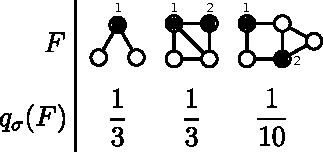
\includegraphics{qsig_example}
    \caption{Flags and their normalising factors}
    \label{fig:qsig_example}
\end{figure}

Now we can define the averaging operator:

\begin{definition}[Averaging Operator]
    \label{def:classic_averaging}
    We define the map $\llbracket \cdot \rrbracket\colon \Acl^\sigma \to \Acl^\emptyset$
    as follows. For a fixed $\sigma$-flag $F$ define
    $\llbracket F \rrbracket := q_\sigma(F) \downflag{F}$.
    We then extend this function linearly to the space
    $\mathcal{A}^\sigma = \R\Gcl^\sigma / \mathcal{K}^\sigma$. This is well defined by
    theorem 2.5 in \cite{razborovFlagAlgebras2007}.
\end{definition}

\begin{note}
    This map $\llbracket \cdot \rrbracket$ is a linear map, but not an algebra homomorphism.
    i.e. We do not have
    $\llbracket f\cdot g \rrbracket = \llbracket f \rrbracket \llbracket g \rrbracket$
    in general.
\end{note}

The following result is the key to linking $\Acl^\sigma \to \Acl^\emptyset$:
\begin{lemma}[Lemma 4 \cite{silvaFlagAlgebrasFirst2016}]
    \label{lemma:classic_exp_flags}
    Let $F$ be a $\sigma$-flag and $G$ a graph with $p(\sigma; G) > 0.$ Then let
    $\theta$ be a uniformly random $\sigma$-embedding into $G$, then:
    \[
        \E_\theta[p(F; (G, \theta)]
        = \frac{p(\llbracket F \rrbracket; G)}{p(\llbracket \sigma \rrbracket; G)}
        = \frac{q_\sigma(F)p(\downflag{F}; G)}{q_\sigma(\sigma)p(\sigma; G)}
    \]
    In particular by linearity of expectation this can be extended
    $\Acl^\sigma$.
\end{lemma}

\begin{note}
    In Razborov's paper he describes (definition 10) a measure theoretic way of constructing
    a random distribution of limit functionals $\psi$ from some fixed limit functional
    $\phi$ in such a way that
    $\E_\psi[\psi(F)] = \frac{\phi(\llbracket f \rrbracket)}{\phi(\sigma)}$.
\end{note}

An important corollary of lemma \ref{lemma:classic_exp_flags} is the following:
\begin{lemma}
    The averaging operator $\llbracket \cdot \rrbracket$ maps $\SemCone^\sigma$ to
    $\SemCone^\emptyset$, meaning it preserves positivity.

    In particular, $\llbracket f^2 \rrbracket \geq 0\ \forall\ f \in\Acl^\sigma$.
\end{lemma}

This gives us yet another important tool to prove results using this algebra. In particular
we are now able to prove Mantel's theorem.

\begin{example}[Proof of Mantel's theorem]
    Let $\Gcl$ be the class of triangle free graphs. Mantel's theorem says that
    $\phi(\edge) \leq \frac{1}{2}\ \forall\ \phi\in\Phi^\emptyset$. We prove this
    by showing $\edge \leq \frac{1}{2}$ meaning $\frac{1}{2}\emptyset - \edge \geq 0$.
    Choosing representatives of the cosets of $\emptyset$ and $\edge$ this is the same
    as showing
    $\frac{1}{2}(\triangletwoedge + \triangleoneedge + \triangleempty) - (\frac{2}{3}\triangletwoedge + \frac{1}{3}\triangleoneedge) \geq 0$.
    Simplifying coefficients this means we need to show
    $-\frac{1}{6}\triangletwoedge + \frac{1}{6}\triangleoneedge + \frac{1}{2}\triangleempty \geq 0$.

    Consider then the type $\sigma=\vertex.$ We must
    have $(\edgemarked -\nonedgemarked)^2\in\SemCone^\sigma$
    so we have
    $\llbracket (\edgemarked-\nonedgemarked)^2\rrbracket \in\SemCone^\emptyset$.
    We can compute that
    $\llbracket (\edgemarked-\nonedgemarked)^2\rrbracket= -\frac{1}{3}\triangletwoedge-\frac{1}{3}\triangleoneedge+\triangleempty$.

    Therefore as $\SemCone^\emptyset$ is a convex cone we have
    $\frac{1}{2}(-\frac{1}{3}\triangletwoedge-\frac{1}{3}\triangleoneedge+\triangleempty) + \frac{1}{3}\triangletwoedge \geq 0$
    which does simplify to exactly
    $-\frac{1}{6}\triangletwoedge + \frac{1}{6}\triangleoneedge + \frac{1}{2}\triangleempty$.
    In one line this is:
    \[\phi(\edge) \leq \phi(\edge + \llbracket (\edgemarked - \nonedgemarked)^2\rrbracket + \frac{1}{3}\triangleoneedge) = \phi(\frac{1}{2}(\triangletwoedge + \triangleoneedge + \triangleempty))=\frac{1}{2}.\]
\end{example}

\section{The Semidefinite Method}
\label{sec:semidefinite_method}

We saw in the previous section that we can derive new true statements about densities
by finding elements of the semantic cone
$\SemCone^\emptyset$, and that taking convex combinations of known
"axiomatic" positive elements is a good way to do that. In general to prove
$\phi(f) \leq \lambda\ \forall\ \phi\in\Phi^\emptyset$
we need to show $\lambda\emptyset - f \geq_{\Acl^\emptyset} 0$. It also
suffices to find $\lambda\emptyset - (f + r) \geq 0$ for some $r \geq 0$.

Given some fixed $f\in\Acl^\sigma$ then we want to solve
$\min\{\lambda\colon \lambda\emptyset - f \in \SemCone^\emptyset\}$.

\subsection{Linear Programming}

One direct way to approach this is to take some fixed set of known positive elements
$v_1, \dots, v_k\in\Acl^\emptyset$ and try to minimise our objective over non-negative linear
combinations of these vectors. This corresponds to a method called \textit{linear programming (LP)}.

Fix our \textit{objective vector} $f\in\Acl^\sigma$.

Take some finite list of flags $F_1, \dots, F_\ell$ such that $v_1, \dots, v_k$ and $f$
can be expressed in the basis $\Bcl = (F_1, \dots, F_l, \emptyset).$
This gives us a notion of a coefficient function $\coef_i$ for each $i\in[\ell]$ and
$\coef_\emptyset$. WLOG $f$ has no $\emptyset$ coefficient.

Then if $c=[c_1, \dots, c_k]^T\in\R^k$ is elementwise non-negative
$\sum_{i=1}^kc_iv_i$ is $\in\SemCone^\emptyset$. We want this to equal some
$\lambda\emptyset - (f+r)$ where $r\in\SemCone^\emptyset$.
Each element of the basis is in the cone so it suffices
to find $c_1, \dots, c_k$ such that $\coef_j(\sum_{i=1}^kc_i v_i) \leq -\coef_j(f)\ \forall\ j\in[\ell]$.
Then our $\lambda$ is given by $\coef_\emptyset(\sum_{i=1}^kc_iv_i)$. We can express
this as an optimisation problem over real matrices.

Construct a matrix $A$ as
\[
    A :=
    \begin{bmatrix}
    \coef_1(v_1) & \coef_2(v_1) & \dots & \coef_\ell(v_1)\\
    \coef_1(v_2) & \coef_2(v_2) & \dots & \coef_\ell(v_2)\\
    \vdots & \vdots & & \vdots\\
    \coef_1(v_k) & \coef_2(v_k) & \dots & \coef_\ell(v_k)\\
    \end{bmatrix}
\]
and let $\beta=[\coef_\emptyset(v_1), \dots, \coef_\emptyset(v_k)]^T\in\R^k$. WLOG
$f$ has no $\emptyset$ component so we write
$f=[\coef_1(f), \dots, \coef_\ell(f)]^T\in\R^\ell$. Then our problem is expressed as:
\[
    \begin{split}
    \min_{c\in\R^k} &\ \ \  c^T\beta\\
    \text{such that} &\ \ \  c^T(-A) \geq f\\
                     &\ \ \  c \geq 0.
    \end{split}
\]
This is the standard form of a linear programming problem. Many fast solvers exist to find
good solutions.

\begin{example}[Proving Mantel's theorem via LP]
    Our objective vector is $f=\frac{2}{3}\triangletwoedge + \frac{1}{3}\triangleoneedge$.
    We can use two known elements of the semantic cone:
    $v_1 = \llbracket (\edgemarked - \nonedgemarked)^2 \rrbracket=\triangleempty - \frac{1}{3}\triangletwoedge - \frac{1}{3}\triangletwoedge$
    and
    $v_2 = \triangleoneedge$.
    We choose $\Bcl=(\triangleoneedge, \triangletwoedge, \emptyset)$ and use the fact that
    $\emptyset = \triangleempty + \triangleoneedge + \triangletwoedge$ to write
    $v_1 = \emptyset - \frac{4}{3}\triangleoneedge - \frac{4}{3}\triangletwoedge$.
    Then in vector notation $f=[\frac{1}{3}, \frac{2}{3}, 0]^T$,
    $v_1 = [-\frac{4}{3}, -\frac{4}{3}, 1]^T$ and
    $v_2 = [1, 0, 0]^T$.
    Then we find
    \[
        A = \begin{bmatrix}
            -\frac{4}{3} & -\frac{4}{3}\\
            1 & 0
        \end{bmatrix}
    \]
    Hence we want to find $c=[c_1, c_2] \geq 0$ such that
    $c(-A) \geq [\frac{1}{3}, \frac{2}{3}]^T$ minimising $c^T[1, 0]^T$.
    It can be found that an optimal solution is $c=[\frac{1}{2}, \frac{1}{3}]^T$
    giving value $\frac{1}{2}$. Hence $\edge \leq \frac{1}{2}$ as expected.
\end{example}

This method works when we have a fixed list of known elements of
$\SemCone^\emptyset$ but how can we incorporate an entire space of these elements?

\subsection{Semidefinite Programming}

TODO REMINDER WHAT IS SEMIDEFINITE MATRIX

We know that $\llbracket \nu^2 \rrbracket \in\SemCone^\emptyset\ \forall\ \nu\in\Acl^\sigma$.
How do we encode this into our optimisation problem?
One way to do this would be to add a search variable for $\nu\in\Acl^\sigma$
and consider $\llbracket \nu^2 \rrbracket$ as one of our known elements of the semantic cone.
i.e. take our list of known positive elements $v_1, \dots, v_k$ then try to
minimise $\sum_{i=1}^kc_i\coef_\emptyset(v_i) + \coef_\emptyset(\llbracket\nu^2\rrbracket)$
over $c\in\R^k, \nu\in\Acl^\sigma$
such that
$c \geq_{\R^k} 0$ and $\sum_{i=1}^k c_i \coef_j(v_i) + \coef_j(\llbracket\nu^2\rrbracket) \leq -\coef_j(f)\ \forall\ j \in[\ell]$.
We can express this in the language of matrices and column vectors.

Assume as before we have a basis $\Bcl = (F_1, \dots, F_\ell, \emptyset)$
of a subspace of $\Acl^\emptyset$ as above. Then for a type $\sigma$ consider some basis
$\Bcl^\sigma=(F_1^\sigma, \dots, F_m^\sigma)$ of $\Acl^\sigma$ such
that $\llbracket \nu^2 \rrbracket \in \spanop\Bcl\ \forall\ \nu\in\spanop\Bcl^\sigma$.

It can be shown then that, as $\llbracket\cdot\rrbracket$ is a linear function and
writing $\nu=\sum_{i=1}^m a_i F_i^\sigma$ we have the following for all $k\in[\ell]$
and similarly for $\coef_\emptyset$.
\[
    \coef_k(\llbracket \nu^2 \rrbracket) = \sum_{i=1}^m\sum_{j=1}^m
    a_ia_j\coef_k(\llbracket F_i^\sigma\cdot F_j^\sigma\rrbracket).
\]
meaning we can define matrices $C^\sigma_i$ for each $i\in[\ell]$ and $C^\sigma_\emptyset$ as
as
\[
    C^\sigma_i :=
    \begin{bmatrix}
    \coef_i(\llbracket (F_1^\sigma)^2 \rrbracket)
    & \coef_i(\llbracket F_1^\sigma F_2^\sigma \rrbracket))
    & \dots
    & \coef_i(\llbracket F_1^\sigma F_m^\sigma \rrbracket)\\
    \coef_i(\llbracket F_2^\sigma F_1^\sigma \rrbracket)
    & \coef_i(\llbracket (F_2^\sigma)^2 \rrbracket))
    & \dots
    & \coef_i(\llbracket F_2^\sigma F_m^\sigma \rrbracket)\\
    \vdots & \vdots & & \vdots\\
    \coef_i(\llbracket F_m^\sigma F_1^\sigma \rrbracket)
    & \coef_i(\llbracket F_m^\sigma F_2^\sigma \rrbracket))
    & \dots
    & \coef_i(\llbracket (F_m^\sigma)^2 \rrbracket)\\
    \end{bmatrix}
\]
and find that $\coef_i(\llbracket \nu^2 \rrbracket) = \nu^T C^\sigma_i \nu$ where
$\nu$ is considered a column vector over $\Bcl^\sigma$. By cyclicity
of the trace we have
$\nu^TC^\sigma_i\nu = \trace(\nu\nu^TC^\sigma_i)=\langle \nu\nu^T, C^\sigma_i\rangle$
where $\langle \cdot \rangle$ is the standard inner product on real symmetric matrices.

The collection of matrices $C^\sigma_i$ are fixed by choice of $\Bcl^\sigma$ so we now know how
to compute
the coefficients of $\llbracket \nu^2\rrbracket$ over $\Bcl$ as the inner product of
$\nu\nu^T$ with some $C^\sigma_i$. The power of this is now we can do better than just searching
over a single vector $\nu$. If we search instead over the space of positive semidefinite (PSD)
matrices then any such $P$ has spectral decomposition $P=\sum_{i=1}^\lambda \nu_i\nu_i^T.$
Then
\[
    \langle P, C^\sigma_i \rangle = \sum_{j=1}^\lambda \langle \nu_j\nu_j^T, C_i^\sigma\rangle
    = \sum_{j=1}^\lambda \coef_i(\llbracket \nu_j^2\rrbracket).
\]
Hence searching over PSD matrices allows us to search over several vectors $\nu_i$ at the
same time. This gives us a new optimisation problem: Given our objective vector
$f\in\Acl^\emptyset$, known elements of the semidefinite cone $v_1, \dots, v_k$,
basis $\Bcl=(F_1, \dots, F_\ell, \emptyset)$ such that $v_1, \dots, v_k, f\in\spanop\Bcl$,
type $\sigma$ and basis $\Bcl^\sigma=(F_1^\sigma, \dots, F_m^\sigma)$ such that
$\llbracket \nu^2\rrbracket\in\spanop\Bcl\ \forall\ \nu\in\spanop\Bcl$ we precompute
the matrices $C_i^\sigma$ for $i\in[\ell]$ and $C_\emptyset$ and then try to solve:
\[
    \begin{split}
    \min_{c\in\R^k, P \in \R^{m\times m}}
        &\ \ \sum_{i=1}^kc_i\coef_\emptyset(v_i) + \langle P, C_\emptyset^\sigma\rangle\\
    \text{such that} &\ \ \sum_{i=1}^kc_i\coef_j(v_i) +
        \langle P, C_j^\sigma\rangle = -f_j
        \ \forall\ j \in [\ell]\\
        &\ \ c_i \geq 0\ \forall\ i\in[k]\\
        &\ \ P \succ 0.
    \end{split}
\]
This is a semidefinite program. It can easily be converted to a more standard form. It
can also easily be extended to more than a single type $\sigma$.

Now we can see how we could have used this approach to prove Mantel's theorem,
showing how optimising over $P$ allows us to discover the vector
$\llbracket (\edgemarked - \nonedgemarked)^2\rrbracket$.

\begin{example}[Proving Mantel's theorem via SDP]
    Let $\sigma=\vertex$ and take the bases
    \[
        \Bcl = (\triangleoneedge, \triangletwoedge, \emptyset)
        \ \ \ \Bcl^\sigma = (\edgemarked, \nonedgemarked)
    \]
    Then we can compute the matrix of all $\llbracket F, G\rrbracket$ for $F, G \in\Bcl^\sigma$:
    \[
    \begin{split}
        \begin{bmatrix}
            \left\llbracket (\edgemarked)^2\right\rrbracket
            & \left\llbracket (\edgemarked)(\nonedgemarked)\right\rrbracket\\
            \left\llbracket (\edgemarked)(\nonedgemarked)\right\rrbracket
            & \left\llbracket (\nonedgemarked)^2\right\rrbracket
        \end{bmatrix}
        & = \begin{bmatrix}
            \left\llbracket \triangletwoedgemarkedcentre\right\rrbracket
            & \left\llbracket \frac{1}{2}\triangleoneedgemarkedleft
            +\frac{1}{2}\triangletwoedgemarkedleft\right\rrbracket\\
            \left\llbracket \frac{1}{2}\triangleoneedgemarkedleft
            +\frac{1}{2}\triangletwoedgemarkedleft\right\rrbracket
            & \left\llbracket \triangleemptymarked + \triangleoneedgemarkedtop\right\rrbracket
        \end{bmatrix}\\
        & = \begin{bmatrix}
            \frac{1}{3}\triangletwoedge
            & \frac{1}{3}\triangleoneedge
            +\frac{1}{3}\triangletwoedge\\
            \frac{1}{3}\triangleoneedge
            +\frac{1}{3}\triangletwoedge
            & \triangleempty + \frac{1}{3}\triangleoneedge
        \end{bmatrix}\\
        & = \begin{bmatrix}
            \frac{1}{3}\triangletwoedge
            & \frac{1}{3}\triangleoneedge
            +\frac{1}{3}\triangletwoedge\\
            \frac{1}{3}\triangleoneedge
            +\frac{1}{3}\triangletwoedge
            & \emptyset-\frac{2}{3}\triangleoneedge-\triangletwoedge
        \end{bmatrix}.
    \end{split}
    \]
    giving us the coefficient matrices
    \[
        C^\sigma_1 = 
        \begin{bmatrix}
            0 & \frac{1}{3}\\
            \frac{1}{3} & -\frac{2}{3}
        \end{bmatrix}
        \ C^\sigma_1 = 
        \begin{bmatrix}
            \frac{1}{3} & \frac{1}{3}\\
            \frac{1}{3} & -1
        \end{bmatrix}
        \ C^\sigma_\emptyset = 
        \begin{bmatrix}
            0 & 0\\
            0 & 1
        \end{bmatrix}.
    \]
    We bring in then a single known element of the semantic cone $v_1 = \triangleoneedge$
    and remembering that our objective vector is
    $f=\frac{2}{3}\triangletwoedge+\frac{1}{3}\triangleoneedge$ we compose the SDP problem
    as outlined above and can use a solver to output $c_1=\frac{1}{3}$ and
    $P=\frac{1}{2}\left(\begin{smallmatrix}1 & -1\\ -1 & 1\end{smallmatrix}\right)\succ 0$.
    Then we can verify that
    $\lambda=c_1\coef_\emptyset(v_1) + \langle P, C_\emptyset^\sigma=\frac{1}{2}$
    as expected and we do satisfy the constraints that
    $c_1\coef_1(v_1) + \langle P, C_1^\sigma \rangle = \frac{1}{3} = -\coef_1(f)$
    and
    $c_2\coef_1(v_1) + \langle P, C_2^\sigma \rangle = \frac{2}{3} = -\coef_2(f)$
    as required.
    Therefore $\frac{1}{2}\emptyset - f \in \SemCone^\emptyset\implies\phi(f)\leq\frac{1}{2}\ \forall\ \phi\in\Phi^\emptyset$ as required.

    This value of $P$ shouldn't be surprising as $P = \frac{1}{2}\nu\nu^T$ where
    $\nu = [1, -1]^T = \edgemarked - \nonedgemarked$ so the "discovered" element of
    the semantic cone was the expected $\llbracket (\edgemarked - \nonedgemarked)^2 \rrbracket$.
\end{example}

\subsection{Duality}

Consider again our linear program: Minimise $\coef_\emptyset(\sum_ic_iv_i)$ over
$c\in\R^k_{\geq 0}$ such that $\coef_j(\sum_ic_iv_i)\leq -\coef_j(f)\ \forall\ j\in[\ell]$
which we expressed as a matrix problem:
Minimise $c^T\beta$ over $c\in\R^k$ such that
$c^T(-A) \geq f$ and $c\geq 0$.

The powerful thing about linear programming is duality. We can convert our minimisation
problem above into a dual maximisation problem which asks us to maximise
$f^Tx$ over $x \in \R^\ell$ such that $x \geq 0$ and $(-A)x \leq \beta$.
By weak duality of linear programming
we know that any solution to this problem is a lower bound to any possible solution to
our original (primal) problem.

We can interpret this maximisation problem in a useful way. We can think of this dual
problem as being a relaxation of the search over possible limit functionals $\phi$.
Take the search vector $x\in\R^\ell$ and construct a linear functional $\phi_x$ on the
space $\spanop\Bcl$ by defining $\phi_x(F_i) := x_i$ and $\phi_x(\emptyset) = 1$, then
linearly extending. We can then see that $x \geq 0$ means $\phi(F_i) \geq 0\ \forall\ i \in[\ell]$
which is a requirement of true limit functionals. Similarly the requirement
that $(-A)x \leq \beta$ corresponds to requiring that $\phi(v_i) \geq 0\ \forall\ i\in[k]$,
meaning our known elements of the semantic cone must have positive value as expected.
Finally then $\max_{x\in\R^\ell} f^Tx$ corresponds to $\max \phi_x(f)$.

Hence the dual problem attempts to maximise some hypothetical $\phi_x(f)$ on the
constraints that $\phi_x$ must behave like a true limit functional. This interpretation
makes it clear that our fixed known elements of the semantic cone correspond to constraints
on the possible space of linear functionals; Adding new positive elements to the list
may exclude previous possible limit functionals and get us closer to a true answer.

We expanded our linear program into a semidefinite program. Luckily for us semidefinite
programs also have duality. The dual version of the SDP above asks us to
maximise $\sum_{x\in\R^\ell}f^Tx$ such that
$\sum_{j=1}^\ell x_j\coef_j(v_i) + \coef_\emptyset(v_i) \geq 0\ \forall\ i\in[k]$ and
$\sum_{j=1}^\ell x_jC_j^\sigma + C_\emptyset^\sigma \succ 0$.

We can again interpret this dual program in the same way, where we take $x\in\R^\ell$,
interpret it as a linear functional $\phi_x$ on $\Bcl$ with $\phi_x(F_i) := x_i$ and
$\phi_x(\emptyset)=1$. Then the dual problem is to maximise $\phi_x(f)$ such that
$\phi(v_i) \geq 0\ \forall\ i\in[k]$ but now we have the additional constraint that
the matrix $Q = \sum_{i=1}^\ell\phi(F_j)C_j^\sigma + C_\emptyset^\sigma$ is positive semidefinite.
But this exactly means that $\nu^T Q \nu \geq 0$ for all $\nu$ which means
$\phi_x(\llbracket \nu^2 \rrbracket) \geq 0\ \forall \nu$. Hence our extension from linear
to semidefinite programming has had the effect on our dual problem of adding the
requirement that $\phi_x(\llbracket \nu^2 \rrbracket) \geq 0$ for all $\nu\in\spanop\Bcl^\sigma$.

This gives us our overall strategy then for using flag algebras and semidefinite programming.
If you want to prove an upper bound on some density function, express it as $\phi(f)$ for
some vector $f$, then generate as many linear constraints on the space of linear functionals
$\phi_x$ as possible and finally add the requirement that $\phi_x(\llbracket \nu^2\rrbracket)\geq 0$
for all $\nu$ in some subspace. Then the problem of maximising $\phi_x(f)$ can be
converted rigorously to a dual problem of finding convex combinations of elements of the
semantic cone, proving true upper bounds on $\phi(f)\forall\phi\in\Phi^\emptyset$.

\section{Coloured Graphs}
\label{sec:coloured_graphs}

We have already discussed graphs with colourings in the introduction. In that context
we were considering some underlying graph $G$ and asking questions about what possible
colourings $G$ can admit under certain constraints. In this section we are going to take
a very different view of graphs and colourings, we instead consider a graphs with colourings
as combinatorial objects in their own right.

\begin{definition}[$(c_v, c_e)$-Graph]
    Given $c_v, c_e \in \N$ where $c_v, c_e \geq 1$ we define a
    \textbf{$(c_v, c_e)$-graph} to be a simple undirected graph where each edge and
    each vertex are assigned colours from $[c_v]$ and $[c_e]$ respectively.

    We often call $(k, 1)$-graphs or $(1,k)$-graphs $k$-vertex-colour graphs or
    $k$-edge-colour graphs respectively.
\end{definition}
\begin{note}
    It's very important to highlight here that we do \textbf{not} require that the colourings
    are proper: Adjacent vertices and incident edges can have the same colour.
\end{note}
\begin{definition}
    Two $(c_e,c_v)$-graphs $G, G'$ are isomorphic if there is a graph isomorphism
    $f\colon G \to G'$ which preserves colours.
\end{definition}

\begin{example}
    A $(2, 1)$-graph is a graph where each vertex can have 1 of 2 colours, and each edge is fixed
    to same colour. We usually visually show colour 1 as black and colour 2 as red. See
    figure \ref{fig:all_2_1_graphs} for all 2-vertex-coloured graphs of size 3.
\end{example}

\begin{figure}[ht]
    \centering
    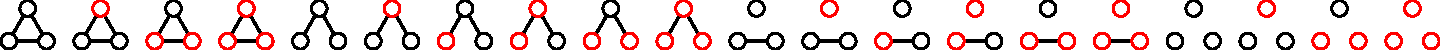
\includegraphics[scale=0.6]{all_2_1_graphs.pdf}
    \caption{All $(2,1)$-graphs of size 3 up to isomorphism}
    \label{fig:all_2_1_graphs}
\end{figure}

\begin{example}
    The category of $(1,1)$-graphs is equivalent to the category of simple graphs.
\end{example}

All of what we have seen in the previous sections applies exactly the same to
coloured graphs as to graphs. We have types and flags and flag algebras in the exact
same way. The induced count function $c(F; G)$ now counts those $U\subseteq V(G)$ such that
$G[U] \cong F$ as coloured graphs.
See figure \ref{fig:coloured_flag_example} for an example expression in $\sigma$-flags derived from
$(2, 2)$-graphs where $\sigma=\redvertex$, a single red vertex (colour 2).

\begin{figure}[ht]
    \centering
    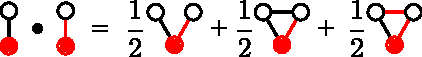
\includegraphics[scale=1.25]{coloured_flag_example}
    \caption{An example expression in an $(2,2)$-graph flag algebra}
    \label{fig:coloured_flag_example}
\end{figure}
